\documentclass[a4paper]{article}
\usepackage[margin=1cm]{geometry}
\usepackage{amsmath, amssymb}
\usepackage{graphicx}
\usepackage{tikz}
\usetikzlibrary{arrows.meta}
\pagestyle{empty}

\definecolor{c0}{HTML}{E53935}
\definecolor{c1}{HTML}{1E88E5}
\definecolor{c2}{HTML}{43A047}
\definecolor{c3}{HTML}{FB8C00}
\definecolor{c4}{HTML}{8E24AA}
\definecolor{c5}{HTML}{00ACC1}
\definecolor{c6}{HTML}{F4511E}
\definecolor{c7}{HTML}{3949AB}
\definecolor{c8}{HTML}{7CB342}
\definecolor{c9}{HTML}{C2185B}
\definecolor{c10}{HTML}{FF7043}
\definecolor{c11}{HTML}{26A69A}
\definecolor{c12}{HTML}{5C6BC0}
\definecolor{c13}{HTML}{FFCA28}
\definecolor{c14}{HTML}{AB47BC}

\begin{document}

\begin{center}
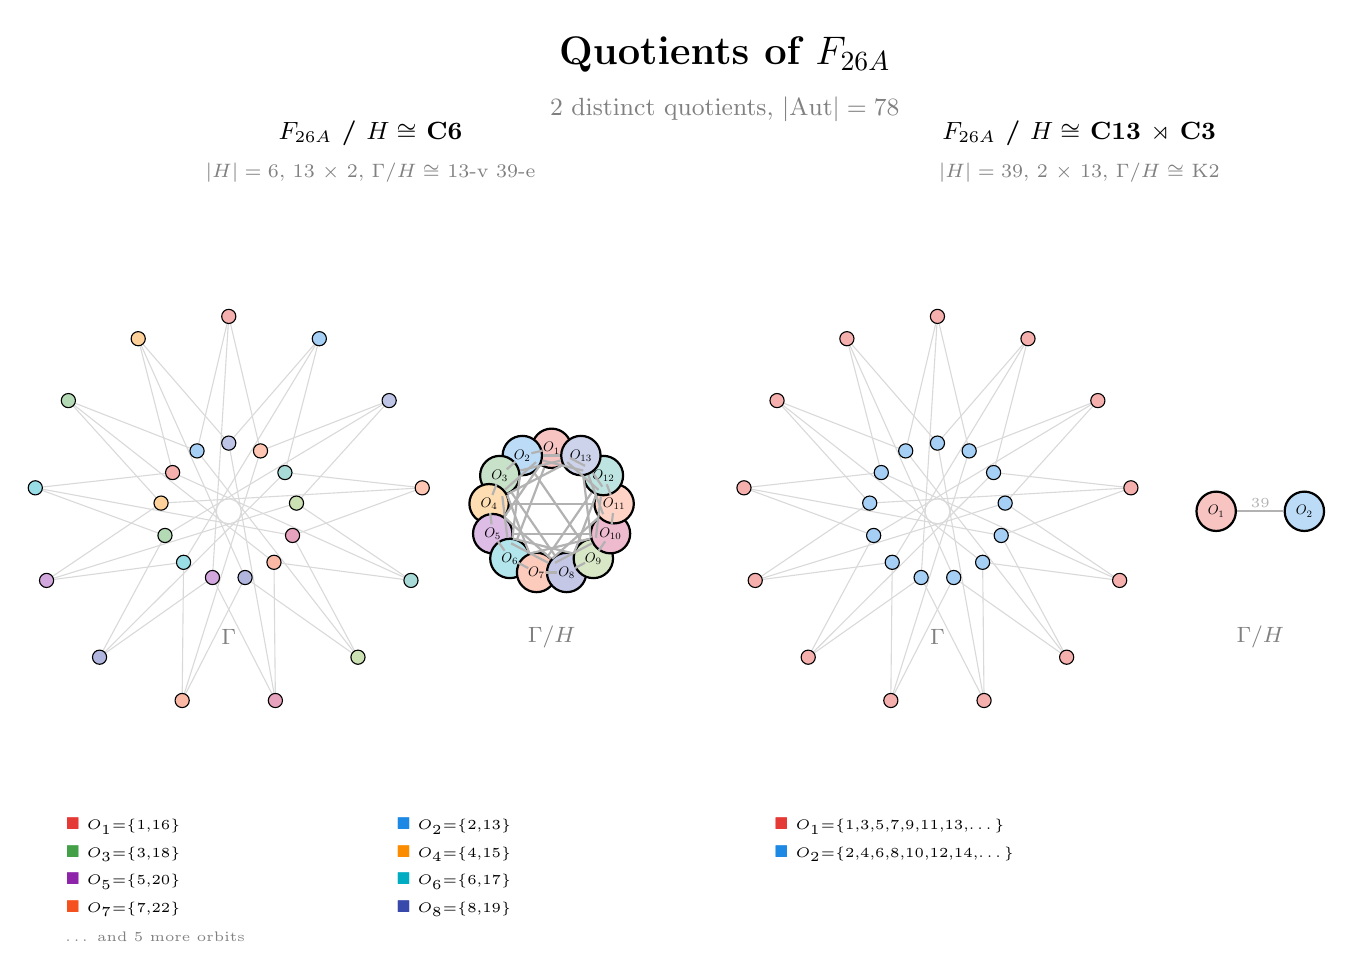
\begin{tikzpicture}[
  ov/.style={circle, draw, semithick, minimum size=3.5mm, inner sep=0pt},
  ovs/.style={circle, draw, thin, minimum size=1.8mm, inner sep=0pt},
  qv/.style={circle, draw, thick, minimum size=5mm, inner sep=0pt},
  cardtitle/.style={font=\small\bfseries},
  cardsub/.style={font=\scriptsize, text=gray},
  glabel/.style={font=\footnotesize, text=gray},
]
\node[font=\Large\bfseries] at (0, 11.5) {Quotients of $F_{26A}$};
\node[font=\small, text=gray] at (0, 10.8) {2 distinct quotients, $|\mathrm{Aut}|=78$};

% Card 1: H=C6
\node[cardtitle] at (-4.50,10.50) {$F_{26A}$ / $H \cong$ C6};
\node[cardsub] at (-4.50,10.00) {$|H|=6$, 13 $\times$ 2, $\Gamma/H \cong$ 13-v 39-e};
\draw[gray!30, thin] (-6.300,8.175) -- (-6.703,6.467);
\draw[gray!30, thin] (-6.300,8.175) -- (-6.507,4.859);
\draw[gray!30, thin] (-6.300,8.175) -- (-5.897,6.467);
\draw[gray!30, thin] (-6.703,6.467) -- (-8.337,7.106);
\draw[gray!30, thin] (-6.703,6.467) -- (-4.659,3.847);
\draw[gray!30, thin] (-8.337,7.106) -- (-7.160,5.804);
\draw[gray!30, thin] (-8.337,7.106) -- (-5.726,5.052);
\draw[gray!30, thin] (-7.160,5.804) -- (-8.614,4.822);
\draw[gray!30, thin] (-7.160,5.804) -- (-3.843,5.998);
\draw[gray!30, thin] (-8.614,4.822) -- (-6.874,5.052);
\draw[gray!30, thin] (-8.614,4.822) -- (-5.440,5.804);
\draw[gray!30, thin] (-6.874,5.052) -- (-6.892,3.297);
\draw[gray!30, thin] (-6.874,5.052) -- (-5.150,7.892);
\draw[gray!30, thin] (-6.892,3.297) -- (-6.093,4.859);
\draw[gray!30, thin] (-6.892,3.297) -- (-5.897,6.467);
\draw[gray!30, thin] (-6.093,4.859) -- (-4.659,3.847);
\draw[gray!30, thin] (-6.093,4.859) -- (-7.450,7.892);
\draw[gray!30, thin] (-4.659,3.847) -- (-5.490,5.393);
\draw[gray!30, thin] (-5.490,5.393) -- (-3.843,5.998);
\draw[gray!30, thin] (-5.490,5.393) -- (-8.757,5.998);
\draw[gray!30, thin] (-3.843,5.998) -- (-5.587,6.192);
\draw[gray!30, thin] (-5.587,6.192) -- (-5.150,7.892);
\draw[gray!30, thin] (-5.587,6.192) -- (-7.941,3.847);
\draw[gray!30, thin] (-5.150,7.892) -- (-6.300,6.566);
\draw[gray!30, thin] (-6.300,6.566) -- (-7.450,7.892);
\draw[gray!30, thin] (-6.300,6.566) -- (-5.708,3.297);
\draw[gray!30, thin] (-7.450,7.892) -- (-7.013,6.192);
\draw[gray!30, thin] (-7.013,6.192) -- (-8.757,5.998);
\draw[gray!30, thin] (-7.013,6.192) -- (-3.986,4.822);
\draw[gray!30, thin] (-8.757,5.998) -- (-7.110,5.393);
\draw[gray!30, thin] (-7.110,5.393) -- (-7.941,3.847);
\draw[gray!30, thin] (-7.110,5.393) -- (-4.263,7.106);
\draw[gray!30, thin] (-7.941,3.847) -- (-6.507,4.859);
\draw[gray!30, thin] (-6.507,4.859) -- (-5.708,3.297);
\draw[gray!30, thin] (-5.708,3.297) -- (-5.726,5.052);
\draw[gray!30, thin] (-5.726,5.052) -- (-3.986,4.822);
\draw[gray!30, thin] (-3.986,4.822) -- (-5.440,5.804);
\draw[gray!30, thin] (-5.440,5.804) -- (-4.263,7.106);
\draw[gray!30, thin] (-4.263,7.106) -- (-5.897,6.467);
\node[ovs, fill=c0!40] at (-6.300,8.175) {};
\node[ovs, fill=c1!40] at (-6.703,6.467) {};
\node[ovs, fill=c2!40] at (-8.337,7.106) {};
\node[ovs, fill=c3!40] at (-7.160,5.804) {};
\node[ovs, fill=c4!40] at (-8.614,4.822) {};
\node[ovs, fill=c5!40] at (-6.874,5.052) {};
\node[ovs, fill=c6!40] at (-6.892,3.297) {};
\node[ovs, fill=c7!40] at (-6.093,4.859) {};
\node[ovs, fill=c8!40] at (-4.659,3.847) {};
\node[ovs, fill=c9!40] at (-5.490,5.393) {};
\node[ovs, fill=c10!40] at (-3.843,5.998) {};
\node[ovs, fill=c11!40] at (-5.587,6.192) {};
\node[ovs, fill=c1!40] at (-5.150,7.892) {};
\node[ovs, fill=c12!40] at (-6.300,6.566) {};
\node[ovs, fill=c3!40] at (-7.450,7.892) {};
\node[ovs, fill=c0!40] at (-7.013,6.192) {};
\node[ovs, fill=c5!40] at (-8.757,5.998) {};
\node[ovs, fill=c2!40] at (-7.110,5.393) {};
\node[ovs, fill=c7!40] at (-7.941,3.847) {};
\node[ovs, fill=c4!40] at (-6.507,4.859) {};
\node[ovs, fill=c9!40] at (-5.708,3.297) {};
\node[ovs, fill=c6!40] at (-5.726,5.052) {};
\node[ovs, fill=c11!40] at (-3.986,4.822) {};
\node[ovs, fill=c8!40] at (-5.440,5.804) {};
\node[ovs, fill=c12!40] at (-4.263,7.106) {};
\node[ovs, fill=c10!40] at (-5.897,6.467) {};
\node[glabel] at (-6.30,4.10) {$\Gamma$};
\node[qv, fill=c0!30] (c0o0) at (-2.200,6.500) {\scalebox{0.5}{$O_{1}$}};
\node[qv, fill=c1!30] (c0o1) at (-2.572,6.408) {\scalebox{0.5}{$O_{2}$}};
\node[qv, fill=c2!30] (c0o2) at (-2.858,6.154) {\scalebox{0.5}{$O_{3}$}};
\node[qv, fill=c3!30] (c0o3) at (-2.994,5.796) {\scalebox{0.5}{$O_{4}$}};
\node[qv, fill=c4!30] (c0o4) at (-2.948,5.416) {\scalebox{0.5}{$O_{5}$}};
\node[qv, fill=c5!30] (c0o5) at (-2.730,5.101) {\scalebox{0.5}{$O_{6}$}};
\node[qv, fill=c6!30] (c0o6) at (-2.391,4.923) {\scalebox{0.5}{$O_{7}$}};
\node[qv, fill=c7!30] (c0o7) at (-2.009,4.923) {\scalebox{0.5}{$O_{8}$}};
\node[qv, fill=c8!30] (c0o8) at (-1.670,5.101) {\scalebox{0.5}{$O_{9}$}};
\node[qv, fill=c9!30] (c0o9) at (-1.452,5.416) {\scalebox{0.5}{$O_{10}$}};
\node[qv, fill=c10!30] (c0o10) at (-1.406,5.796) {\scalebox{0.5}{$O_{11}$}};
\node[qv, fill=c11!30] (c0o11) at (-1.542,6.154) {\scalebox{0.5}{$O_{12}$}};
\node[qv, fill=c12!30] (c0o12) at (-1.828,6.408) {\scalebox{0.5}{$O_{13}$}};
\draw[gray!60, thick] (c0o0) -- (c0o1);
\draw[gray!60, thick] (c0o0) -- (c0o3);
\draw[gray!60, thick] (c0o0) -- (c0o4);
\draw[gray!60, thick] (c0o0) -- (c0o5);
\draw[gray!60, thick] (c0o0) -- (c0o10);
\draw[gray!60, thick] (c0o0) -- (c0o11);
\draw[gray!60, thick] (c0o1) -- (c0o2);
\draw[gray!60, thick] (c0o1) -- (c0o5);
\draw[gray!60, thick] (c0o1) -- (c0o8);
\draw[gray!60, thick] (c0o1) -- (c0o11);
\draw[gray!60, thick] (c0o1) -- (c0o12);
\draw[gray!60, thick] (c0o2) -- (c0o3);
\draw[gray!60, thick] (c0o2) -- (c0o5);
\draw[gray!60, thick] (c0o2) -- (c0o6);
\draw[gray!60, thick] (c0o2) -- (c0o7);
\draw[gray!60, thick] (c0o2) -- (c0o12);
\draw[gray!60, thick] (c0o3) -- (c0o4);
\draw[gray!60, thick] (c0o3) -- (c0o7);
\draw[gray!60, thick] (c0o3) -- (c0o10);
\draw[gray!60, thick] (c0o3) -- (c0o12);
\draw[gray!60, thick] (c0o4) -- (c0o5);
\draw[gray!60, thick] (c0o4) -- (c0o7);
\draw[gray!60, thick] (c0o4) -- (c0o8);
\draw[gray!60, thick] (c0o4) -- (c0o9);
\draw[gray!60, thick] (c0o5) -- (c0o6);
\draw[gray!60, thick] (c0o5) -- (c0o9);
\draw[gray!60, thick] (c0o6) -- (c0o7);
\draw[gray!60, thick] (c0o6) -- (c0o9);
\draw[gray!60, thick] (c0o6) -- (c0o10);
\draw[gray!60, thick] (c0o6) -- (c0o11);
\draw[gray!60, thick] (c0o7) -- (c0o8);
\draw[gray!60, thick] (c0o7) -- (c0o11);
\draw[gray!60, thick] (c0o8) -- (c0o9);
\draw[gray!60, thick] (c0o8) -- (c0o11);
\draw[gray!60, thick] (c0o8) -- (c0o12);
\draw[gray!60, thick] (c0o9) -- (c0o10);
\draw[gray!60, thick] (c0o9) -- (c0o12);
\draw[gray!60, thick] (c0o10) -- (c0o11);
\draw[gray!60, thick] (c0o10) -- (c0o12);
\node[glabel] at (-2.20,4.10) {$\Gamma/H$};
\node[anchor=west, font=\tiny] at (-8.50,1.70) {\textcolor{c0}{$\blacksquare$} $O_{1}$=\{1,16\}};
\node[anchor=west, font=\tiny] at (-4.30,1.70) {\textcolor{c1}{$\blacksquare$} $O_{2}$=\{2,13\}};
\node[anchor=west, font=\tiny] at (-8.50,1.35) {\textcolor{c2}{$\blacksquare$} $O_{3}$=\{3,18\}};
\node[anchor=west, font=\tiny] at (-4.30,1.35) {\textcolor{c3}{$\blacksquare$} $O_{4}$=\{4,15\}};
\node[anchor=west, font=\tiny] at (-8.50,1.00) {\textcolor{c4}{$\blacksquare$} $O_{5}$=\{5,20\}};
\node[anchor=west, font=\tiny] at (-4.30,1.00) {\textcolor{c5}{$\blacksquare$} $O_{6}$=\{6,17\}};
\node[anchor=west, font=\tiny] at (-8.50,0.65) {\textcolor{c6}{$\blacksquare$} $O_{7}$=\{7,22\}};
\node[anchor=west, font=\tiny] at (-4.30,0.65) {\textcolor{c7}{$\blacksquare$} $O_{8}$=\{8,19\}};
\node[anchor=west, font=\tiny, text=gray] at (-8.50,0.30) {\ldots\ and 5 more orbits};

% Card 2: H=C13 : C3
\node[cardtitle] at (4.50,10.50) {$F_{26A}$ / $H \cong$ C13 $\rtimes$ C3};
\node[cardsub] at (4.50,10.00) {$|H|=39$, 2 $\times$ 13, $\Gamma/H \cong$ K2};
\draw[gray!30, thin] (2.700,8.175) -- (2.297,6.467);
\draw[gray!30, thin] (2.700,8.175) -- (2.493,4.859);
\draw[gray!30, thin] (2.700,8.175) -- (3.103,6.467);
\draw[gray!30, thin] (2.297,6.467) -- (0.663,7.106);
\draw[gray!30, thin] (2.297,6.467) -- (4.341,3.847);
\draw[gray!30, thin] (0.663,7.106) -- (1.840,5.804);
\draw[gray!30, thin] (0.663,7.106) -- (3.274,5.052);
\draw[gray!30, thin] (1.840,5.804) -- (0.386,4.822);
\draw[gray!30, thin] (1.840,5.804) -- (5.157,5.998);
\draw[gray!30, thin] (0.386,4.822) -- (2.126,5.052);
\draw[gray!30, thin] (0.386,4.822) -- (3.560,5.804);
\draw[gray!30, thin] (2.126,5.052) -- (2.108,3.297);
\draw[gray!30, thin] (2.126,5.052) -- (3.850,7.892);
\draw[gray!30, thin] (2.108,3.297) -- (2.907,4.859);
\draw[gray!30, thin] (2.108,3.297) -- (3.103,6.467);
\draw[gray!30, thin] (2.907,4.859) -- (4.341,3.847);
\draw[gray!30, thin] (2.907,4.859) -- (1.550,7.892);
\draw[gray!30, thin] (4.341,3.847) -- (3.510,5.393);
\draw[gray!30, thin] (3.510,5.393) -- (5.157,5.998);
\draw[gray!30, thin] (3.510,5.393) -- (0.243,5.998);
\draw[gray!30, thin] (5.157,5.998) -- (3.413,6.192);
\draw[gray!30, thin] (3.413,6.192) -- (3.850,7.892);
\draw[gray!30, thin] (3.413,6.192) -- (1.059,3.847);
\draw[gray!30, thin] (3.850,7.892) -- (2.700,6.566);
\draw[gray!30, thin] (2.700,6.566) -- (1.550,7.892);
\draw[gray!30, thin] (2.700,6.566) -- (3.292,3.297);
\draw[gray!30, thin] (1.550,7.892) -- (1.987,6.192);
\draw[gray!30, thin] (1.987,6.192) -- (0.243,5.998);
\draw[gray!30, thin] (1.987,6.192) -- (5.014,4.822);
\draw[gray!30, thin] (0.243,5.998) -- (1.890,5.393);
\draw[gray!30, thin] (1.890,5.393) -- (1.059,3.847);
\draw[gray!30, thin] (1.890,5.393) -- (4.737,7.106);
\draw[gray!30, thin] (1.059,3.847) -- (2.493,4.859);
\draw[gray!30, thin] (2.493,4.859) -- (3.292,3.297);
\draw[gray!30, thin] (3.292,3.297) -- (3.274,5.052);
\draw[gray!30, thin] (3.274,5.052) -- (5.014,4.822);
\draw[gray!30, thin] (5.014,4.822) -- (3.560,5.804);
\draw[gray!30, thin] (3.560,5.804) -- (4.737,7.106);
\draw[gray!30, thin] (4.737,7.106) -- (3.103,6.467);
\node[ovs, fill=c0!40] at (2.700,8.175) {};
\node[ovs, fill=c1!40] at (2.297,6.467) {};
\node[ovs, fill=c0!40] at (0.663,7.106) {};
\node[ovs, fill=c1!40] at (1.840,5.804) {};
\node[ovs, fill=c0!40] at (0.386,4.822) {};
\node[ovs, fill=c1!40] at (2.126,5.052) {};
\node[ovs, fill=c0!40] at (2.108,3.297) {};
\node[ovs, fill=c1!40] at (2.907,4.859) {};
\node[ovs, fill=c0!40] at (4.341,3.847) {};
\node[ovs, fill=c1!40] at (3.510,5.393) {};
\node[ovs, fill=c0!40] at (5.157,5.998) {};
\node[ovs, fill=c1!40] at (3.413,6.192) {};
\node[ovs, fill=c0!40] at (3.850,7.892) {};
\node[ovs, fill=c1!40] at (2.700,6.566) {};
\node[ovs, fill=c0!40] at (1.550,7.892) {};
\node[ovs, fill=c1!40] at (1.987,6.192) {};
\node[ovs, fill=c0!40] at (0.243,5.998) {};
\node[ovs, fill=c1!40] at (1.890,5.393) {};
\node[ovs, fill=c0!40] at (1.059,3.847) {};
\node[ovs, fill=c1!40] at (2.493,4.859) {};
\node[ovs, fill=c0!40] at (3.292,3.297) {};
\node[ovs, fill=c1!40] at (3.274,5.052) {};
\node[ovs, fill=c0!40] at (5.014,4.822) {};
\node[ovs, fill=c1!40] at (3.560,5.804) {};
\node[ovs, fill=c0!40] at (4.737,7.106) {};
\node[ovs, fill=c1!40] at (3.103,6.467) {};
\node[glabel] at (2.70,4.10) {$\Gamma$};
\node[qv, fill=c0!30] (c1o0) at (6.240,5.700) {\scalebox{0.5}{$O_{1}$}};
\node[qv, fill=c1!30] (c1o1) at (7.360,5.700) {\scalebox{0.5}{$O_{2}$}};
\draw[gray!60, thick] (c1o0) -- node[font=\tiny, auto, inner sep=1pt] {39} (c1o1);
\node[glabel] at (6.80,4.10) {$\Gamma/H$};
\node[anchor=west, font=\tiny] at (0.50,1.70) {\textcolor{c0}{$\blacksquare$} $O_{1}$=\{1,3,5,7,9,11,13,\ldots\}};
\node[anchor=west, font=\tiny] at (0.50,1.35) {\textcolor{c1}{$\blacksquare$} $O_{2}$=\{2,4,6,8,10,12,14,\ldots\}};
\end{tikzpicture}
\end{center}

\end{document}